\documentclass[12pt,twoside]{article}
%\usepackage[table]{xcolor} % important to avoid options clash.
%\input{02465shared_preamble}
%\usepackage{cleveref}
\usepackage{url}
\usepackage{graphics}
\usepackage{multicol}
\usepackage{rotate}
\usepackage{rotating}
\usepackage{booktabs}
\usepackage{hyperref}
\usepackage{pifont}
\usepackage{latexsym}
\usepackage[english]{babel}
\usepackage{epstopdf}
\usepackage{etoolbox}
\usepackage{amsmath}
\usepackage{amssymb}
\usepackage{multirow,epstopdf}
\usepackage{fancyhdr}
\usepackage{booktabs}
\usepackage{xcolor}
\newcommand\redt[1]{ {\textcolor[rgb]{0.60, 0.00, 0.00}{\textbf{ #1} } } }


\newcommand{\m}[1]{\boldsymbol{ #1}}
\newcommand{\yoursolution}{ \redt{(your solution here) } } 



\title{ Report 2 hand-in }
\date{ \today }
\author{Alice (\texttt{s000001})\and  Bob (\texttt{s000002})\and Clara (\texttt{s000003}) } 

\begin{document}
\maketitle

\begin{table}[ht!]
\caption{Attribution table. Feel free to add/remove rows and columns}
\begin{tabular}{llll}
\toprule
                                                                    & Alice   & Bob    & Clara   \\
\midrule
 1: Formulate Yodas pendulum as a linear problem                    & 0-100\%  & 0-100\% & 0-100\%  \\
 2: Build a PID controller to stop Master Yodas pendulum            & 0-100\%  & 0-100\% & 0-100\%  \\
 3: Optimal LQR to stop the pendulum                                & 0-100\%  & 0-100\% & 0-100\%  \\
 4: PID corresponding to optimal controller                         & 0-100\%  & 0-100\% & 0-100\%  \\
 5: Reflect on PID controller                                       & 0-100\%  & 0-100\% & 0-100\%  \\
 6: State at a later time                                           & 0-100\%  & 0-100\% & 0-100\%  \\
 7: State at a later time II                                        & 0-100\%  & 0-100\% & 0-100\%  \\
 8: Eigenvalues and powers                                          & 0-100\%  & 0-100\% & 0-100\%  \\
 9: Analytical expression of Eigenvalues using Euler discretization & 0-100\%  & 0-100\% & 0-100\%  \\
 10: Bound using Euler discretization                               & 0-100\%  & 0-100\% & 0-100\%  \\
 11: Matrix norm of Exponential discretization (harder)             & 0-100\%  & 0-100\% & 0-100\%  \\
 12: Stability                                                      & 0-100\%  & 0-100\% & 0-100\%  \\
 13: Discretization                                                 & 0-100\%  & 0-100\% & 0-100\%  \\
 14: Linearization                                                  & 0-100\%  & 0-100\% & 0-100\%  \\
 15: Unitgrade self-check                                           & 0-100\%  & 0-100\% & 0-100\%  \\
 16: Optimal planning                                               & 0-100\%  & 0-100\% & 0-100\%  \\
 17: Control using simple linearization                             & 0-100\%  & 0-100\% & 0-100\%  \\
 18: MPC                                                            & 0-100\%  & 0-100\% & 0-100\%  \\
\bottomrule
\end{tabular}
\end{table}

%\paragraph{Statement about collaboration:}
%Please edit this section to reflect how you have used external resources. The following statement will in most cases suffice: 
%\emph{The code in the irls/project1 directory is entirely}

%\paragraph{Main report:}
Headings have been inserted in the document for readability. You only have to edit the part which says \yoursolution. 

\section{Master Yodas pendulum (\texttt{yoda\_part1.py})}\label{yoda1}
\subsubsection*{{\color{red}Problem 1:  Formulate Yodas pendulum as a linear problem}}
	
	\begin{align}
		A & = \begin{bmatrix} \cdots \\ \cdots \end{bmatrix}  \\
		B & = \dots 		
	\end{align}
	\yoursolution 	
	
\subsubsection*{{\color{red}Problem 2:  Build a PID controller to stop Master Yodas pendulum}}

	$$
x^* = \cdot, \quad	K_d = \cdot, \quad K_p = \cdot, \quad K_I=\cdot
	$$
\begin{center}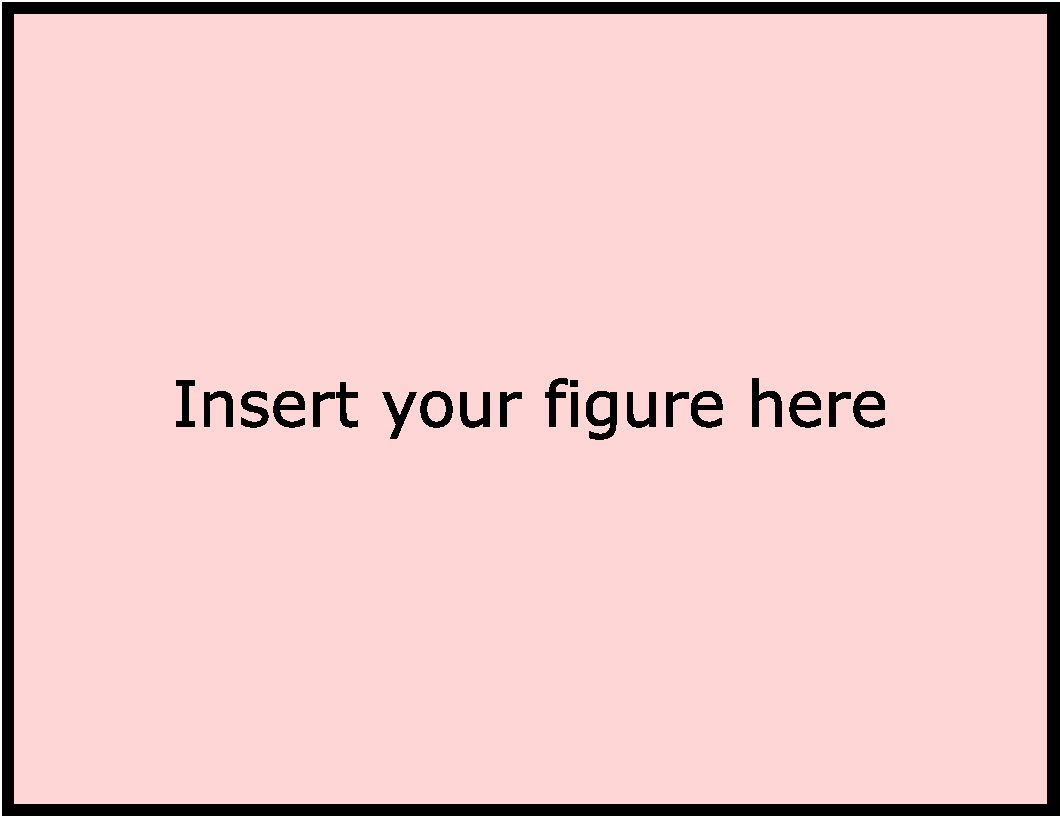
\includegraphics[width=.8\linewidth]{figures/your_answer} \end{center}
\yoursolution	

\subsubsection*{{\color{red}Problem 5:  Reflect on PID controller}}
			
		\begin{center}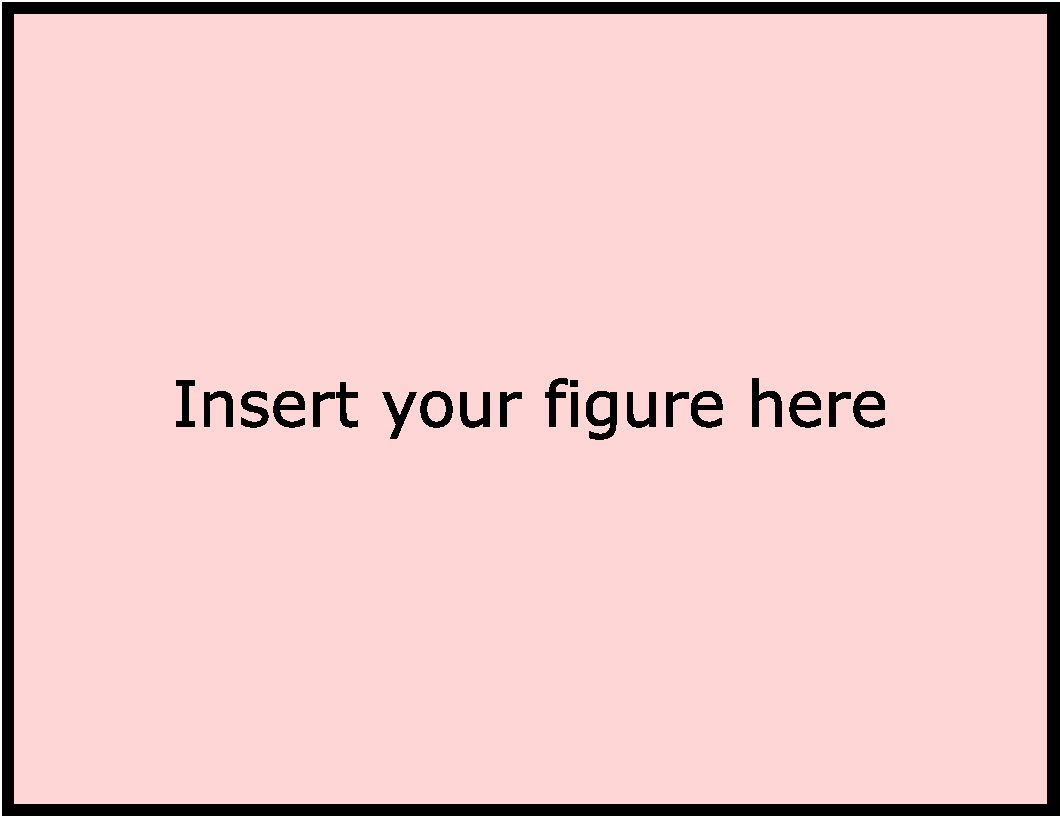
\includegraphics[width=.6\linewidth]{figures/your_answer} \end{center}
	The two action sequences differs because... \yoursolution	
	
\section{Yodas pendulum revisited \texttt{yoda\_part2.py} }\label{yoda2}
\subsubsection*{{\color{red}Problem 6:  State at a later time}}
	
		To solve the first part, we can write $\m x_N = ...$ 
		
		As for the second part we get:
\begin{align}
\tilde A_0 & = \cdots, \quad A_0 = \cdots
\end{align}
		\yoursolution 	
\subsubsection*{{\color{red}Problem 8:  Eigenvalues and powers}}
	
Assume $\lambda_1, \lambda_2$ are the eigenvalues ... then the Eigenvalues of $M$ is ... similarly for $\tilde M$ ... 
\yoursolution
	
\subsubsection*{{\color{red}Problem 9:  Analytical expression of Eigenvalues using Euler discretization}}

... we get a characteristic polynomial of ... and therefore it follows from Mat1 that the two Eigenvalues are ... 
\yoursolution

\subsubsection*{{\color{red}Problem 10:  Bound using Euler discretization}}

	Using Euler discretization we get the upper bound:
	$$
\| \m x_N \| \leq \cdots
$$
\yoursolution
	
\subsubsection*{{\color{red}Problem 11:  Matrix norm of Exponential discretization (harder)}}
	
Using exponential discretization we get an upper bound of:
		$$
		\| \m x_N \| \leq \cdots
		$$
		\yoursolution
	
\section{R2D2 and control (\texttt{r2d2.py})}
\subsubsection*{{\color{red}Problem 13:  Discretization}}

	$$
	\m x_{k+1} = \m f_k(\m x_k, \m u_k) = \begin{bmatrix} \cdots \\ \cdots \\ \cdots \end{bmatrix}$$

\subsubsection*{{\color{red}Problem 14:  Linearization}}
	
$$
		\m x_{k+1} \approx \begin{bmatrix} \cdots \\ \cdots \\ \cdots \end{bmatrix} \m x_k + 
		\begin{bmatrix} \cdots \\ \cdots \\ \cdots \end{bmatrix} \m u_k +  
		\begin{bmatrix} \vdots \end{bmatrix} 
$$
	
\subsubsection*{{\color{red}Problem 16:  Optimal planning}}
		
	\begin{center}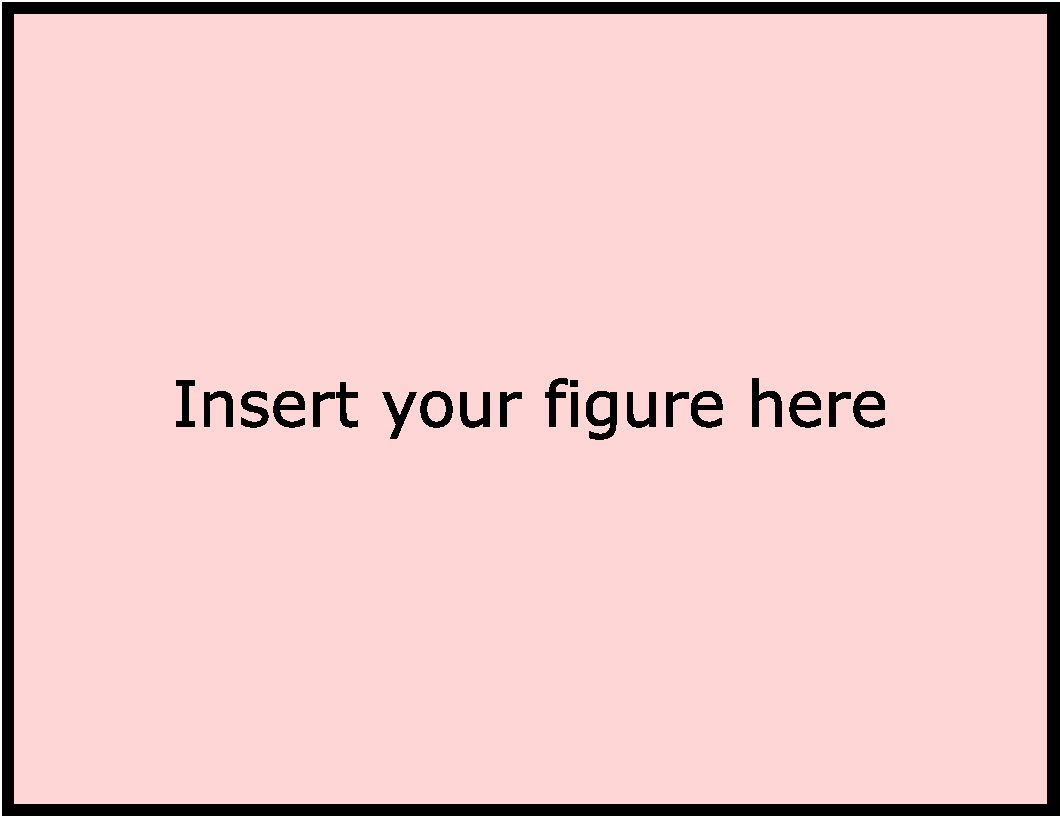
\includegraphics[width=.5\linewidth]{figures/your_answer}~
		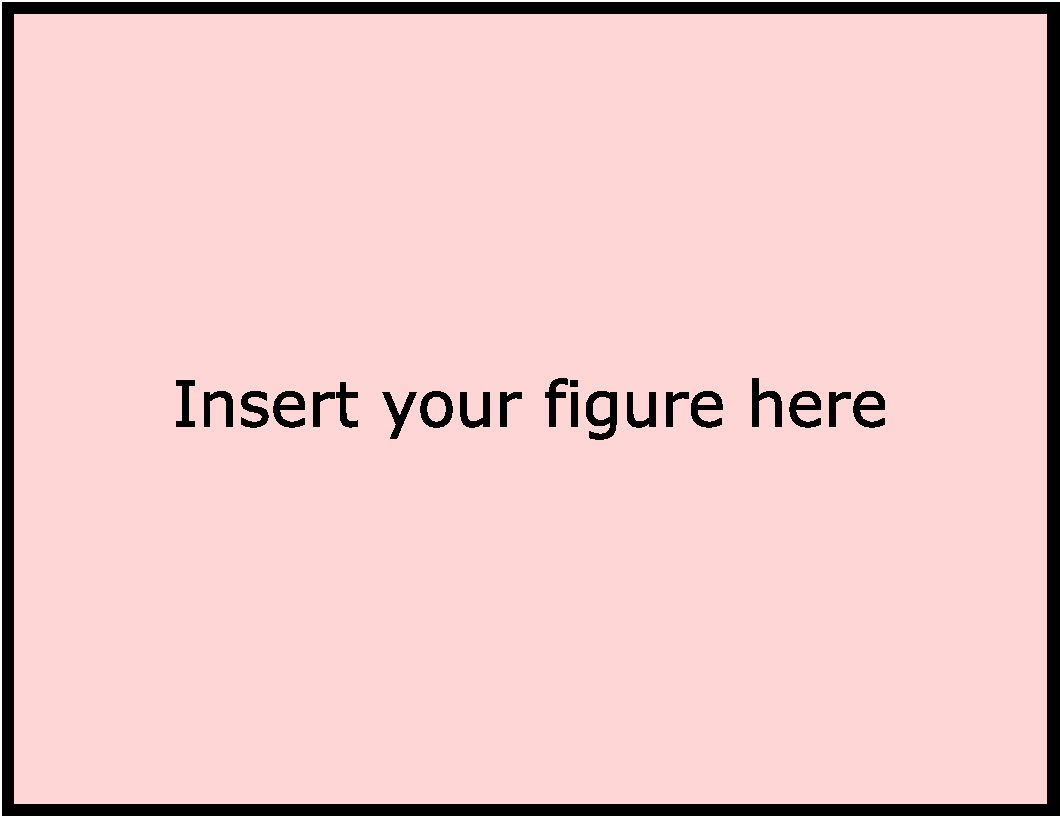
\includegraphics[width=.5\linewidth]{figures/your_answer} \end{center}

\subsubsection*{{\color{red}Problem 17:  Control using simple linearization}}
			
		% Just generate the figures using the script and change the path below. 
		\begin{center}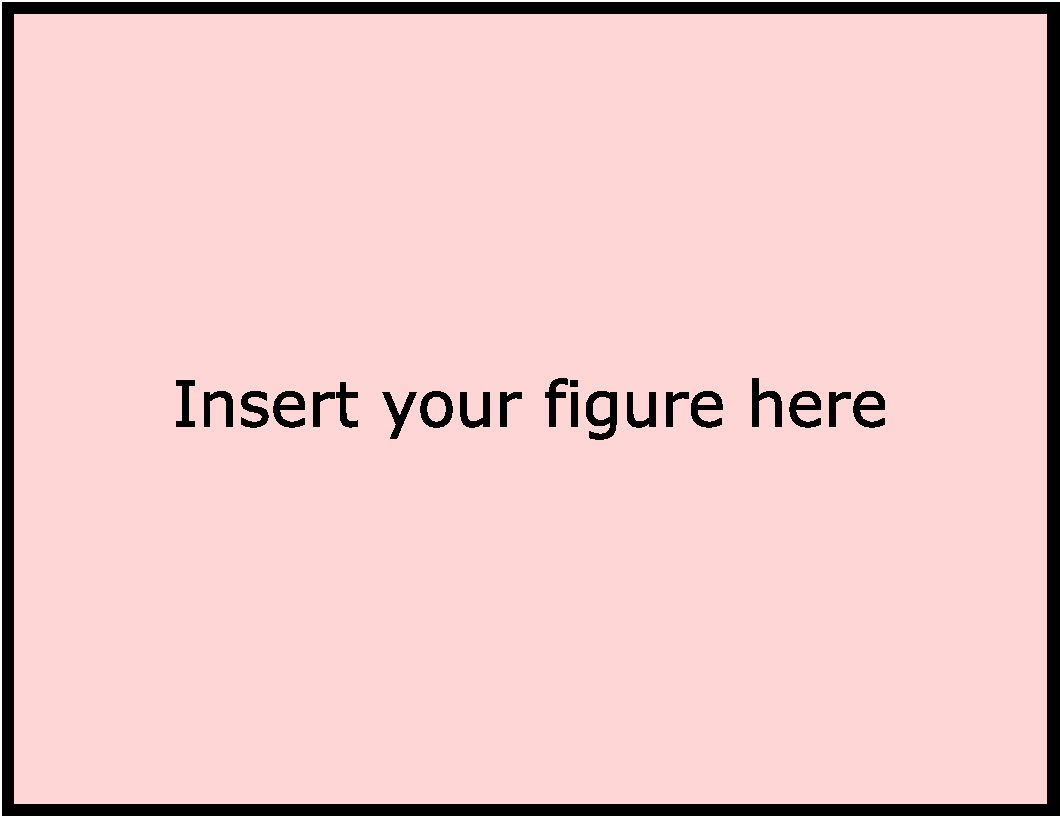
\includegraphics[width=.5\linewidth]{figures/your_answer}~
		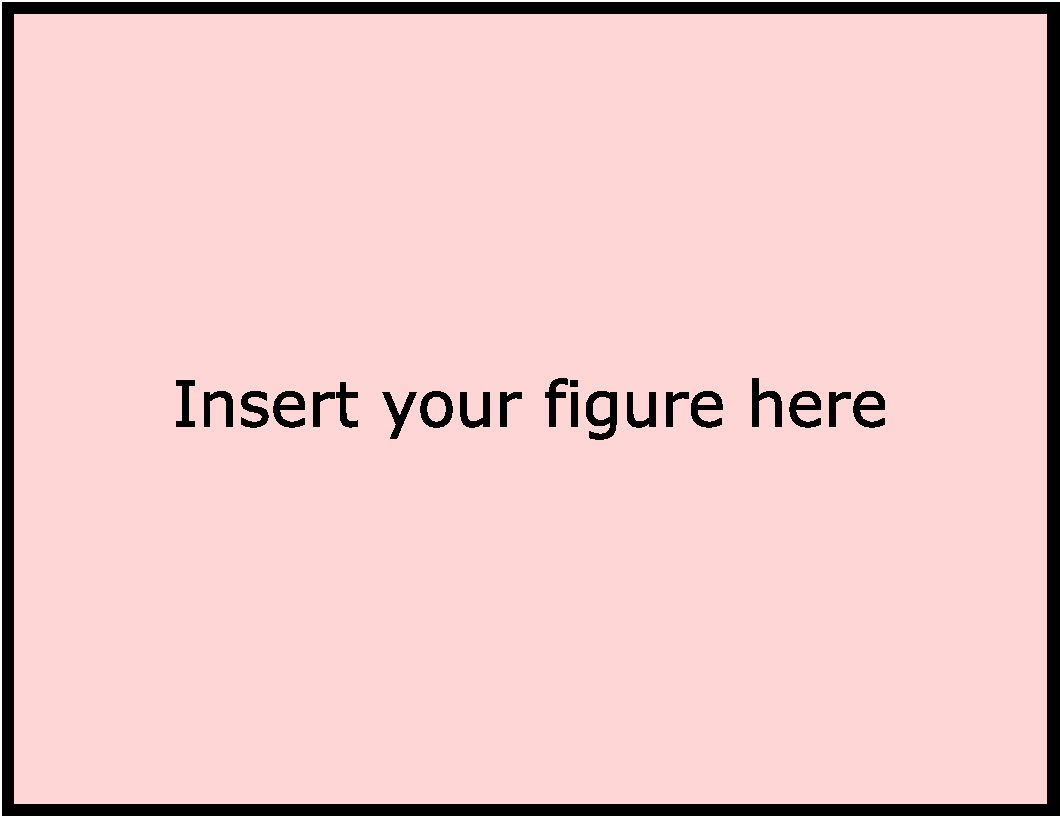
\includegraphics[width=.5\linewidth]{figures/your_answer} \end{center}
Intuitively, the second case fails because... \yoursolution	
	
\subsubsection*{{\color{red}Problem 18:  MPC}}
			
		\begin{center}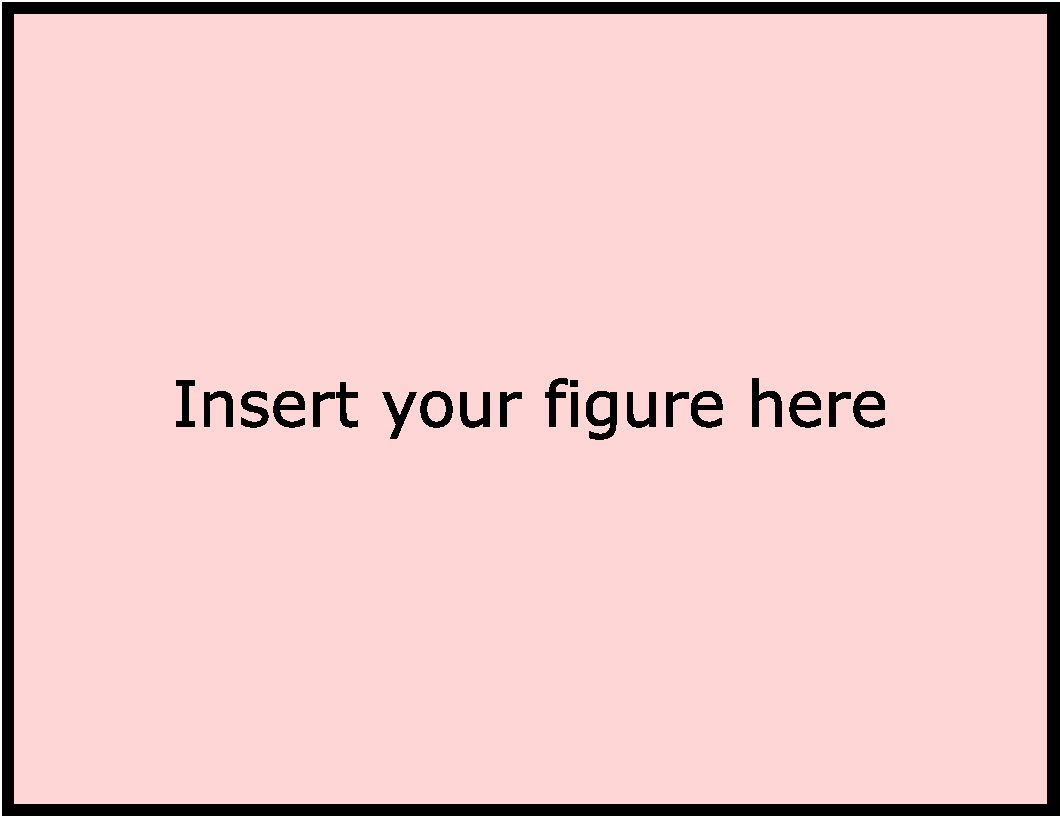
\includegraphics[width=.8\linewidth]{figures/your_answer}%~
		%	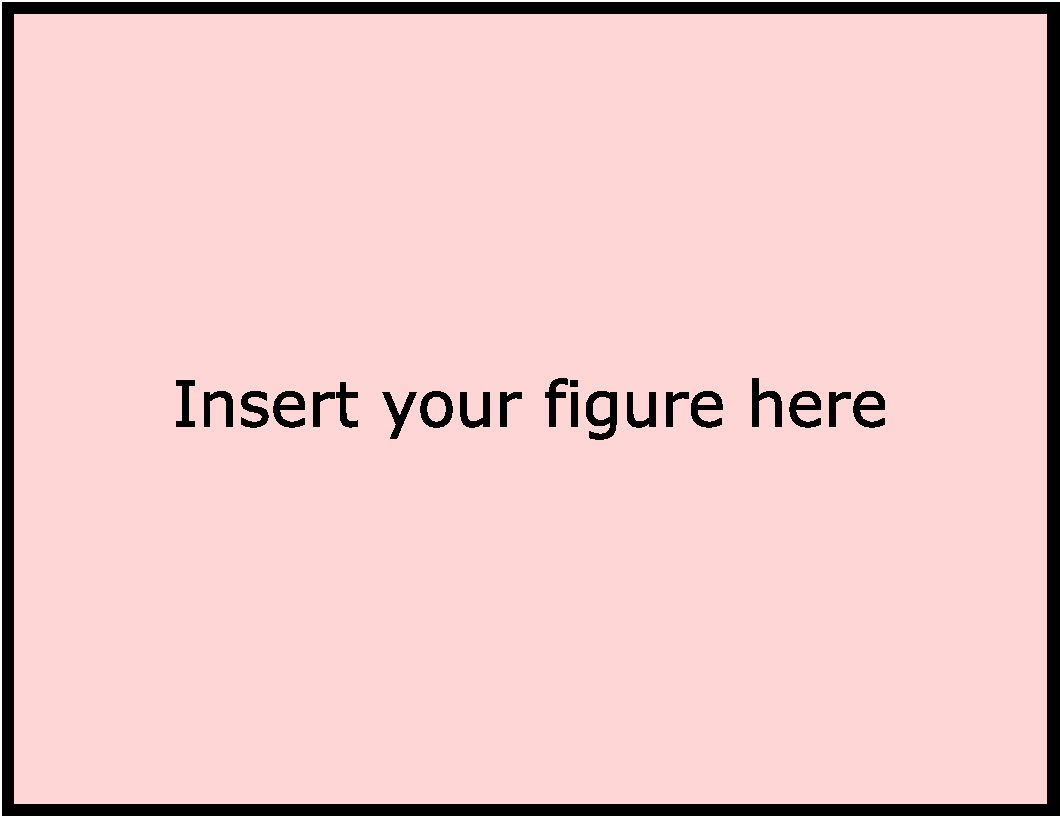
\includegraphics[width=.5\linewidth]{figures/your_answer} 
	\end{center}
		Iterative linearization solves the problem because... \yoursolution
	
\end{document}